\documentclass[aspectratio=169,14pt]{beamer}
\usetheme{default}\usecolortheme{default}\setbeamertemplate{navigation symbols}{}
\setbeamertemplate{footline}{\hfill{\scriptsize\color{covermuted}\insertframenumber/\inserttotalframenumber}\hspace{0.4cm}\vspace{0.15cm}}
\usepackage{fontspec}\usepackage{xeCJK}\setCJKmainfont{PingFang SC}[BoldFont=PingFang SC Semibold]\setmainfont{Helvetica Neue}[BoldFont=Helvetica Neue Bold]
\usepackage{xcolor}\usepackage{tikz}\usepackage{graphicx}\usepackage{fontawesome5}\usetikzlibrary{positioning,calc,arrows.meta,shadows}
\definecolor{bgmain}{RGB}{238,243,252}\definecolor{panel}{RGB}{238,244,255}\definecolor{factbg}{RGB}{246,242,235}\definecolor{coverprimary}{HTML}{2563EB}\definecolor{coveraccent}{HTML}{00A884}\definecolor{coverwarning}{HTML}{F59E0B}\definecolor{coverdark}{HTML}{1F2937}\definecolor{covermuted}{HTML}{64748B}\definecolor{titlecolor}{RGB}{30,30,30}\definecolor{muteddark}{RGB}{72,86,115}\definecolor{bluepanel}{RGB}{226,237,255}\definecolor{greenpanel}{RGB}{225,246,237}\definecolor{amberpanel}{RGB}{255,244,222}\definecolor{purplepanel}{RGB}{239,231,255}\setbeamercolor{background canvas}{bg=bgmain}
\newcommand{\plainbar}{\begin{tikzpicture}[remember picture, overlay]\fill[coverdark, opacity=0.07] (current page.south west) rectangle ([yshift=0.4cm]current page.south east);\draw[coveraccent, opacity=0.45, line width=0.8pt] ([yshift=0.4cm]current page.south west) -- ([yshift=0.4cm]current page.south east);\end{tikzpicture}}
\newcommand{\deckbackground}{\begin{tikzpicture}[remember picture, overlay]\fill[coverprimary!8] (current page.north west) rectangle (current page.south east);\fill[coverprimary!14] (current page.north west) ++(1.55,-1.35) circle (2.45cm);\fill[coveraccent!12] (current page.south east) ++(-1.9,1.45) circle (2.70cm);\fill[coverwarning!12] (current page.north east) ++(-2.9,-1.8) circle (0.85cm);\foreach \x in {-0.2,0.8,...,16.2} {\draw[coverprimary, opacity=0.045, line width=0.25pt] ([xshift=\x cm]current page.south west) -- ([xshift=\x cm]current page.north west);}\foreach \y in {-0.2,0.7,...,9.3} {\draw[coverprimary, opacity=0.04, line width=0.25pt] ([yshift=\y cm]current page.south west) -- ([yshift=\y cm]current page.south east);}\draw[coveraccent, opacity=0.38, line width=1.1pt] ([xshift=0.35cm,yshift=7.72cm]current page.south west) -- ++(3.25,0) -- ++(0.45,-0.45) -- ++(2.0,0);\draw[coverprimary, opacity=0.24, line width=1.0pt] ([xshift=9.35cm,yshift=8.25cm]current page.south west) -- ++(2.3,0) -- ++(0.55,-0.55) -- ++(3.2,0);\fill[coverdark, opacity=0.07] (current page.south west) rectangle ([yshift=0.42cm]current page.south east);\end{tikzpicture}}
\newcommand{\sectiontitle}[2]{\vspace{-0.52cm}\begin{center}{\fontsize{20}{24}\selectfont\bfseries\color{titlecolor} #1}\\[2pt]{\fontsize{9}{11}\selectfont\itshape\color{muteddark} #2}\end{center}\vspace{0.12cm}}
\newcommand{\portraitbox}[2]{\begin{tikzpicture}\node[draw=coverprimary!28, line width=0.7pt, fill=white, rounded corners=3pt, inner sep=2.5pt, drop shadow={shadow xshift=0.5pt, shadow yshift=-0.5pt, opacity=0.12}] {\includegraphics[width=2.4cm,height=2.9cm,keepaspectratio]{#1}};\end{tikzpicture}{\par\vspace{1pt}\fontsize{6.5}{7.5}\selectfont\color{covermuted} #2\par}}
\newcommand{\placeholderportrait}[2]{\begin{tikzpicture}\node[draw=coverprimary!28, line width=0.7pt, fill=white, rounded corners=3pt, inner sep=2.5pt, drop shadow={shadow xshift=0.5pt, shadow yshift=-0.5pt, opacity=0.12}] {\begin{tikzpicture}\fill[bluepanel] (0,0) rectangle (2.4,2.9);\foreach \x/\y in {0.25/0.45,0.55/1.85,0.95/1.15,1.35/2.2,1.75/0.85,2.1/1.65} {\fill[coverprimary!32] (\x,\y) circle (0.055cm);}\draw[coveraccent!45, line width=0.55pt] (0.25,0.45) -- (0.55,1.85) -- (0.95,1.15) -- (1.35,2.2) -- (1.75,0.85) -- (2.1,1.65);\node[circle, fill=coverprimary!16, minimum size=0.78cm] at (1.2,1.78) {};\node[rounded corners=8pt, fill=coverprimary!16, minimum width=1.28cm, minimum height=0.72cm] at (1.2,0.78) {};\node[font=\fontsize{12}{14}\selectfont\bfseries, text=coverprimary!75!black] at (1.2,0.17) {#1};\end{tikzpicture}};\end{tikzpicture}{\par\vspace{1pt}\fontsize{6.5}{7.5}\selectfont\color{covermuted} #2\par}}
\newcommand{\personslide}[9]{\begin{frame}\plainbar\vspace{-0.45cm}\begin{center}{\fontsize{22}{26}\selectfont\bfseries\color{coverdark} #1}\\[2pt]{\fontsize{9.5}{11.5}\selectfont\color{muteddark} #2}\end{center}\vspace{0.15cm}\begin{columns}[c]\begin{column}{0.22\textwidth}\centering #3\end{column}\begin{column}{0.28\textwidth}\begin{tikzpicture}\node[fill=greenpanel, rounded corners=4pt, inner xsep=6pt, inner ysep=5pt, text width=3.8cm, align=left] {{\fontsize{7}{8.5}\selectfont\bfseries\color{coveraccent!70!black} 获奖}\enspace{\fontsize{7}{8.5}\selectfont\color{coverdark!85} #4}\\[2.5pt]{\fontsize{7}{8.5}\selectfont\bfseries\color{coveraccent!70!black} 生卒}\enspace{\fontsize{7}{8.5}\selectfont\color{coverdark!85} #5}\\[2.5pt]{\fontsize{7}{8.5}\selectfont\bfseries\color{coveraccent!70!black} 身份}\enspace{\fontsize{7}{8.5}\selectfont\color{coverdark!85} #6}\\[2.5pt]{\fontsize{7}{8.5}\selectfont\bfseries\color{coveraccent!70!black} 机构}\enspace{\fontsize{7}{8.5}\selectfont\color{coverdark!85} #7}};\end{tikzpicture}\end{column}\begin{column}{0.48\textwidth}\begin{tikzpicture}\node[draw=coverprimary!35, fill=bluepanel, rounded corners=5pt, inner sep=7pt, text width=6.6cm, anchor=north west] at (0,0) {{\fontsize{8.6}{10.2}\selectfont\bfseries\color{coverprimary!82!black} 核心贡献}\\[3pt]{\fontsize{7.4}{9.2}\selectfont\color{coverdark!84} #8\\[3pt]\textbf{一句话：} #9}};\end{tikzpicture}\end{column}\end{columns}\end{frame}}
\begin{document}
\begin{frame}[plain]
\deckbackground
\begin{tikzpicture}[remember picture, overlay]
  \node[anchor=center, font=\fontsize{28}{34}\selectfont\bfseries, text=coverdark] at ([yshift=2.05cm]current page.center) {沃尔夫数学奖人物谱系};
  \node[anchor=center, font=\fontsize{15}{19}\selectfont, text=coverprimary!82!black] at ([yshift=0.86cm]current page.center) {第8集 \enspace·\enspace 数论、自守形式与 Langlands};
  \node[anchor=center, font=\fontsize{12}{16}\selectfont\bfseries, text=coveraccent!76!black] at ([yshift=0.10cm]current page.center) {Number Theory · Automorphic Forms · Langlands};
  \draw[coveraccent, line width=1.4pt] ([yshift=-1.02cm, xshift=-4.55cm]current page.center) -- ([yshift=-1.02cm, xshift=4.55cm]current page.center);
  \node[anchor=center] at ([yshift=-1.90cm]current page.center) {\begin{tikzpicture}\node[rounded corners=8pt, fill=coverprimary!10, inner sep=4pt, minimum height=1.2em, font=\scriptsize\bfseries, text=coverprimary!85!black] at (-5.30,0) {Siegel};\node[rounded corners=8pt, fill=coverprimary!10, inner sep=4pt, minimum height=1.2em, font=\scriptsize\bfseries, text=coverprimary!85!black] at (-3.79,0) {Selberg};\node[rounded corners=8pt, fill=coverprimary!10, inner sep=4pt, minimum height=1.2em, font=\scriptsize\bfseries, text=coverprimary!85!black] at (-2.27,0) {Piatetski-Shapiro};\node[rounded corners=8pt, fill=coverprimary!10, inner sep=4pt, minimum height=1.2em, font=\scriptsize\bfseries, text=coverprimary!85!black] at (-0.76,0) {Langlands};\node[rounded corners=8pt, fill=coverprimary!10, inner sep=4pt, minimum height=1.2em, font=\scriptsize\bfseries, text=coverprimary!85!black] at (0.76,0) {Wiles};\node[rounded corners=8pt, fill=coverprimary!10, inner sep=4pt, minimum height=1.2em, font=\scriptsize\bfseries, text=coverprimary!85!black] at (2.27,0) {Tate};\node[rounded corners=8pt, fill=coverprimary!10, inner sep=4pt, minimum height=1.2em, font=\scriptsize\bfseries, text=coverprimary!85!black] at (3.79,0) {Sarnak};\node[rounded corners=8pt, fill=coverprimary!10, inner sep=4pt, minimum height=1.2em, font=\scriptsize\bfseries, text=coverprimary!85!black] at (5.30,0) {Arthur};\end{tikzpicture}};
\end{tikzpicture}
\end{frame}
\begin{frame}\plainbar\sectiontitle{数论、自守形式与 Langlands}{Number Theory · Automorphic Forms · Langlands}\begin{center}\begin{tikzpicture}
  \node[draw=coverprimary!45, fill=bluepanel, rounded corners=5pt, inner sep=8pt, text width=11.2cm, align=left] at (0,1.05) {{\fontsize{8.3}{10}\selectfont\bfseries\color{coverprimary!80!black} 本集主线}\\[3pt]{\fontsize{7.4}{9.2}\selectfont\color{coverdark!84} 本集从古典数论与 Siegel 定理，到 Selberg 迹公式、自守形式、L 函数、Langlands 纲领、费马大定理和 Arthur-Selberg 迹公式。}};
  \node[draw=coverwarning!60, fill=amberpanel, rounded corners=5pt, inner sep=7pt, text width=11.2cm, align=center] at (0,-1.45) {{\fontsize{8.0}{9.8}\selectfont\bfseries\color{coverwarning!62!black} 开场问题}\\[-1pt]{\fontsize{7.4}{9}\selectfont\color{coverdark!82} 素数、L 函数和表示论为什么会成为同一套语言？}};
\end{tikzpicture}\end{center}\end{frame}
\begin{frame}\plainbar\sectiontitle{人物路线图}{从早期奠基到现代前沿}\begin{center}\begin{tikzpicture}[milestone/.style={draw=coverprimary!45, fill=panel, rounded corners=4pt, inner xsep=4.0pt, inner ysep=5pt, align=center, font=\fontsize{5.7}{7.0}\selectfont\bfseries}, arrow/.style={-{Stealth}, draw=coveraccent, line width=0.7pt}]
\node[milestone, fill=bluepanel] (m0) at (-5.50,1.0) {1978\\Siegel};
\node[milestone, fill=greenpanel] (m1) at (-3.93,1.0) {1986\\Selberg};
\draw[arrow] (m0) -- (m1);
\node[milestone, fill=amberpanel] (m2) at (-2.36,1.0) {1990\\Piatetski-Shapiro};
\draw[arrow] (m1) -- (m2);
\node[milestone, fill=purplepanel] (m3) at (-0.79,1.0) {1995/96\\Langlands};
\draw[arrow] (m2) -- (m3);
\node[milestone, fill=bluepanel] (m4) at (0.79,1.0) {1995/96\\Wiles};
\draw[arrow] (m3) -- (m4);
\node[milestone, fill=greenpanel] (m5) at (2.36,1.0) {2002/03\\Tate};
\draw[arrow] (m4) -- (m5);
\node[milestone, fill=amberpanel] (m6) at (3.93,1.0) {2014\\Sarnak};
\draw[arrow] (m5) -- (m6);
\node[milestone, fill=purplepanel] (m7) at (5.50,1.0) {2015\\Arthur};
\draw[arrow] (m6) -- (m7);
  \node[draw=coverprimary!38, fill=white, rounded corners=5pt, inner sep=7pt, text width=11.4cm, align=left] at (0,-1.25) {{\fontsize{8.0}{9.8}\selectfont\bfseries\color{coverprimary!80!black} 叙事线}\\[-1pt]{\fontsize{7.2}{8.8}\selectfont\color{coverdark!82} 本集从古典数论与 Siegel 定理，到 Selberg 迹公式、自守形式、L 函数、Langlands 纲领、费马大定理和 Arthur-Selberg 迹公式。}};
\end{tikzpicture}\end{center}\end{frame}
\begin{frame}\plainbar\sectiontitle{本集的四个关键词}{观众需要记住的结构性线索}\begin{columns}[T]
\begin{column}{0.49\textwidth}\begin{tikzpicture}
\node[draw=coverprimary!45, fill=bluepanel, rounded corners=5pt, inner sep=7pt, text width=6.0cm, anchor=north west] at (0,0) {{\fontsize{8.5}{10}\selectfont\bfseries\color{coverprimary!80!black} 1. L 函数}\\[2pt]{\fontsize{7.3}{8.8}\selectfont\color{coverdark!82} 把算术信息编码进解析对象。}};
\node[draw=coverprimary!45, fill=greenpanel, rounded corners=5pt, inner sep=7pt, text width=6.0cm, anchor=north west] at (0,-2.25) {{\fontsize{8.5}{10}\selectfont\bfseries\color{coveraccent!70!black} 2. 迹公式}\\[2pt]{\fontsize{7.3}{8.8}\selectfont\color{coverdark!82} 在谱理论和数论之间架桥。}};
\end{tikzpicture}\end{column}
\begin{column}{0.49\textwidth}\begin{tikzpicture}
\node[draw=coverprimary!45, fill=amberpanel, rounded corners=5pt, inner sep=7pt, text width=6.0cm, anchor=north west] at (0,0) {{\fontsize{8.5}{10}\selectfont\bfseries\color{coverwarning!62!black} 3. 自守形式}\\[2pt]{\fontsize{7.3}{8.8}\selectfont\color{coverdark!82} 对称性、分析和算术的交汇点。}};
\node[draw=coverprimary!45, fill=purplepanel, rounded corners=5pt, inner sep=7pt, text width=6.0cm, anchor=north west] at (0,-2.25) {{\fontsize{8.5}{10}\selectfont\bfseries\color{coverprimary!74!black} 4. Langlands}\\[2pt]{\fontsize{7.3}{8.8}\selectfont\color{coverdark!82} 连接 Galois 表示与自守表示的宏大纲领。}};
\end{tikzpicture}\end{column}\end{columns}\end{frame}
\personslide
  {Carl Ludwig Siegel}
  {卡尔·路德维希·西格尔：古典数论与解析方法}
  {\portraitbox{images/Siegel.jpeg}{Photo: Wikipedia}}
  {1978（82岁）}
  {1896--1981}
  {西德}
  {University of Göttingen}
  {Siegel 在数论、多复变函数和天体力学中贡献重大，Siegel 定理和 Siegel 模形式影响深远。}
  {他代表了古典数论与分析方法的高峰。}
\personslide
  {Atle Selberg}
  {阿特勒·塞尔伯格：筛法与迹公式}
  {\portraitbox{images/Selberg.jpg}{Photo: Wikipedia}}
  {1986（69岁）}
  {1917--2007}
  {挪威/美国}
  {Institute for Advanced Study}
  {Selberg 在筛法、Selberg 迹公式和黎曼 zeta 函数研究中贡献核心，是菲尔兹奖得主。}
  {他的迹公式把谱、几何和数论连成一体。}
\personslide
  {Ilya Piatetski-Shapiro}
  {伊利亚·皮亚捷茨基-沙皮罗：自守形式与 L 函数}
  {\portraitbox{images/PiatetskiShapiro.jpg}{Photo: Wikipedia}}
  {1990（61岁）}
  {1929--2009}
  {苏联/以色列/美国}
  {Tel Aviv University / Yale}
  {Piatetski-Shapiro 在自守形式、L 函数和表示论中贡献深远，是现代 Langlands 方向的重要推动者。}
  {他把表示论语言深深嵌入现代数论。}
\personslide
  {Robert Langlands}
  {罗伯特·朗兰兹：Langlands 纲领}
  {\portraitbox{images/Langlands.jpg}{Photo: Wikipedia}}
  {1995/96（59岁）}
  {1936--}
  {加拿大/美国}
  {Institute for Advanced Study}
  {Langlands 提出连接数论、表示论、调和分析和几何的 Langlands 纲领；2018 年获阿贝尔奖。}
  {他提出了现代数论最宏大的统一蓝图。}
\personslide
  {Andrew Wiles}
  {安德鲁·怀尔斯：费马大定理}
  {\portraitbox{images/Wiles.jpg}{Photo: Wikipedia}}
  {1995/96（42岁）}
  {1953--}
  {英国}
  {Princeton University}
  {Wiles 证明费马大定理，依靠椭圆曲线、模形式和 Galois 表示之间的深层联系；2016 年获阿贝尔奖。}
  {一个古老问题的解决，显示了现代数论体系的力量。}
\personslide
  {John Tate}
  {约翰·泰特：Tate 论题与现代算术几何}
  {\portraitbox{images/Tate.jpg}{Photo: Wikipedia}}
  {2002/03（77岁）}
  {1925--2019}
  {美国}
  {University of Texas at Austin}
  {Tate 的工作深刻影响数论和算术几何，包括 Tate 论题、Tate-Shafarevich 群和 Galois 上同调；2010 年获阿贝尔奖。}
  {他的名字出现在现代数论的许多基本对象上。}
\personslide
  {Peter Sarnak}
  {彼得·萨纳克：自守形式与随机矩阵}
  {\portraitbox{images/Sarnak.jpg}{Photo: Wikipedia}}
  {2014（60岁）}
  {1953--}
  {南非/美国}
  {Princeton University / IAS}
  {Sarnak 在数论、自守形式、谱理论和随机矩阵理论与数论的联系中贡献突出。}
  {他展示了谱、随机性和算术之间的深层共振。}
\personslide
  {James Arthur}
  {詹姆斯·阿瑟：Arthur-Selberg 迹公式}
{\portraitbox{images/Arthur.jpeg}{Photo: Wikipedia / NRJ 2013}}
  {2015（70岁）}
  {1944--}
  {加拿大}
  {University of Toronto}
  {Arthur 发展 Arthur-Selberg 迹公式和自守表示理论，对 Langlands 纲领有基础性贡献。}
  {他把迹公式打磨成现代自守表示理论的核心机器。}
\begin{frame}\plainbar\sectiontitle{第8集的主线}{数论、自守形式与 Langlands}\begin{center}\begin{tikzpicture}[block/.style={draw=coverprimary!42, fill=white, rounded corners=5pt, inner sep=6pt, text width=3.0cm, align=center, font=\fontsize{7.0}{8.5}\selectfont}, arrow/.style={->, draw=coveraccent, line width=0.85pt}]
  \node[block, fill=bluepanel] (a) at (-4.9,1.25) {\textbf{起点}\\基础语言}; \node[block, fill=greenpanel] (b) at (-1.65,1.25) {\textbf{工具}\\结构方法}; \node[block, fill=amberpanel] (c) at (1.65,1.25) {\textbf{突破}\\核心定理}; \node[block, fill=purplepanel] (d) at (4.9,1.25) {\textbf{影响}\\跨域应用};
  \draw[arrow] (a) -- (b); \draw[arrow] (b) -- (c); \draw[arrow] (c) -- (d);
  \node[draw=coverwarning!65, fill=factbg, rounded corners=5pt, inner sep=7pt, text width=11.1cm, align=left] at (0,-1.35) {{\fontsize{8.0}{9.8}\selectfont\bfseries\color{coverwarning!62!black} 一句话总结}\\[-1pt]{\fontsize{7.4}{9}\selectfont\color{coverdark!84} 本集从古典数论与 Siegel 定理，到 Selberg 迹公式、自守形式、L 函数、Langlands 纲领、费马大定理和 Arthur-Selberg 迹公式。}};
\end{tikzpicture}\end{center}\end{frame}
\begin{frame}\plainbar\sectiontitle{下一步}{专题系列衔接}\begin{center}\begin{tikzpicture}
  \node[draw=coverwarning!60, fill=coverwarning!12, rounded corners=5pt, inner sep=7pt, text width=10.5cm, align=center] at (0,1.4) {{\fontsize{8.4}{10}\selectfont\bfseries\color{coverwarning!65!black} 下一集：代数几何、Hodge 理论与表示论}\\[-1pt]{\fontsize{7.4}{9}\selectfont\color{coverdark!80} 继续沿着沃尔夫奖人物谱系，进入下一条数学主线。}};
  \node[draw=coverprimary!45, fill=bluepanel, rounded corners=5pt, inner sep=8pt, text width=10.5cm, align=center] at (0,-1.35) {{\fontsize{10.5}{12.8}\selectfont\bfseries\color{coverprimary!82!black} Kodaira、Deligne、Griffiths、Mumford、Sato、Beilinson、Drinfeld、Lusztig}};
\end{tikzpicture}\end{center}\end{frame}
\end{document}
